\documentclass[../main.tex]{subfiles}
%!TEX root = ./analysisGondolaArm.tex
\graphicspath {{../}}

\begin{document}
\subsection{Gondola Arm Stresses} \label{bearingArm}

\begin{figure}[H]
	\centering
	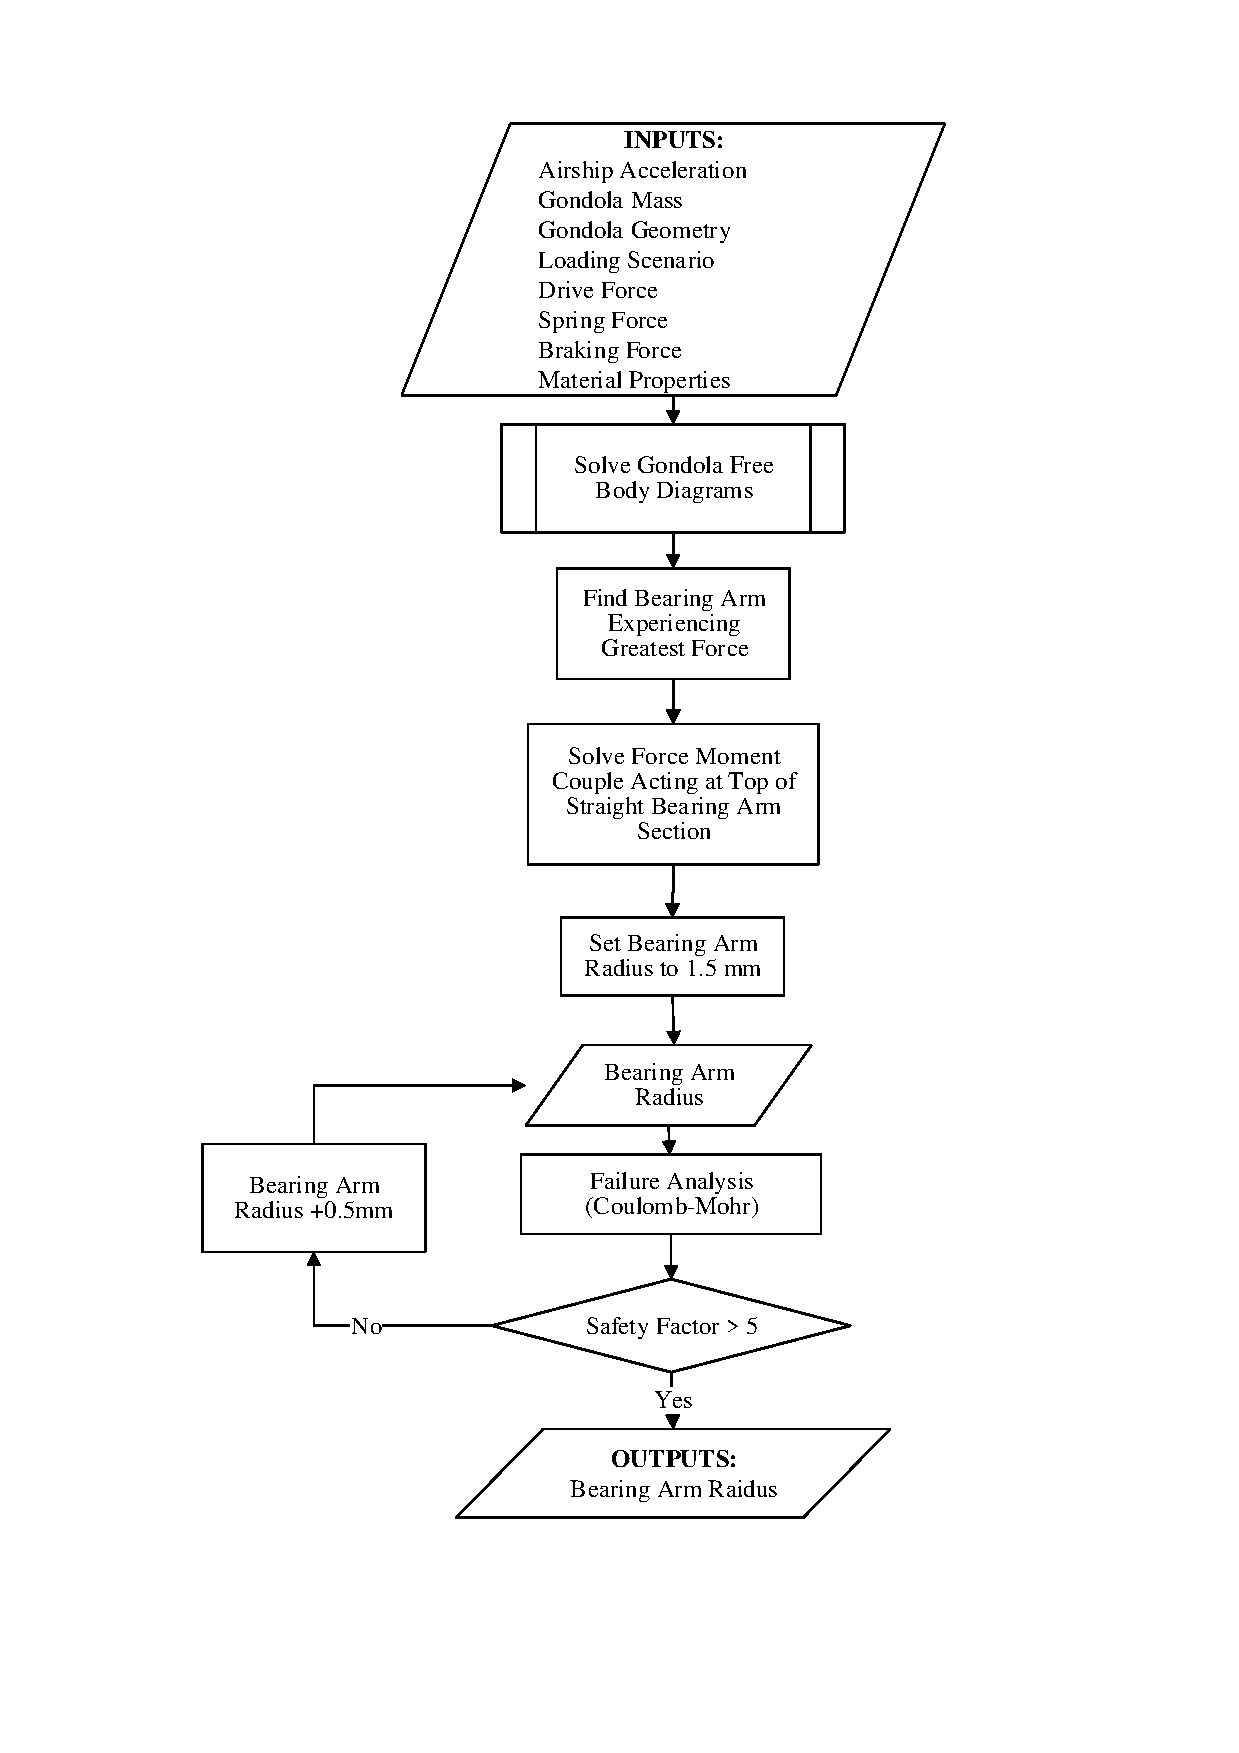
\includegraphics[width=.7\linewidth]{img/paramaterization/gondolaArms.pdf}
	\caption{Parametrization Outline for the Gondola Arms}
	\label{fig:gondolaArmParametrization}
\end{figure}

The failure of the gondola arm will be analysed as shown in Figure \ref{fig:deflection}. 

\begin{figure}[H]
	\centering
	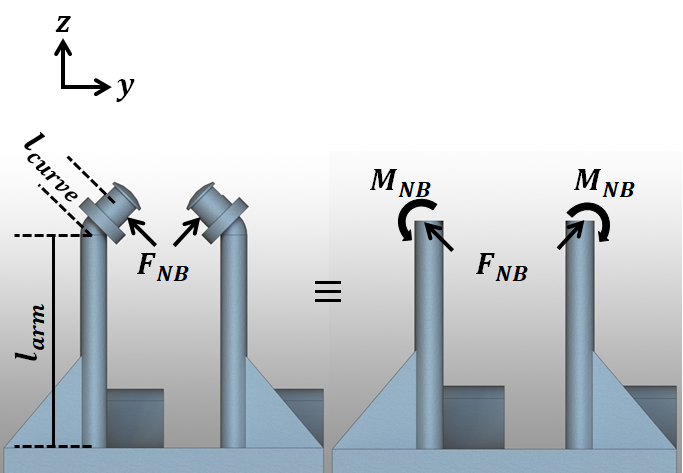
\includegraphics[width=.8\linewidth]{img/gondola/armDeflection.PNG}
	\caption{Model Used to Compute the Deflection of the Gondola Arms}
	\label{fig:deflection}
\end{figure}

For the sake of simplicity, the curved section at the very top is ignored and the force is translated from the curved section to the straight section using a force-moment couple. The moment $M_{NB}$ is computed as $M_{NB}=F_{NB}l_{curve}$. Furthermore, the rib seen in Figure \ref{fig:deflection} is ignored. The failure criteria will be computed without the rib, and the rib will be added as an extra preventative measure, to ensure the member is rigid enough.\\

Three analysis were done on the gondola bearing arms. these include deflection, stress concentration analysis and fatigue analysis. However, the only analysis whose results influenced a change in design was the stress concentration. The other two can be found in Appendix sections \ref{gondDeflection} and \ref{armFatigue}.

The analysis first must solve the gondola forces for the case in which the greatest force is exerted on the bearing arms, when the brake is activated and the airship is thrusting upwards while the pitch remains at 0. This case is explained in System Modeling section \ref{loadingScenarios}, Maximum Bearing Arm Force, and Figure \ref{fig:scenario2}. The forces acting on the gondola in this scenario can be seen in Figure \ref{fig:sideGondolaLA}
\begin{figure}[H]
	\centering
	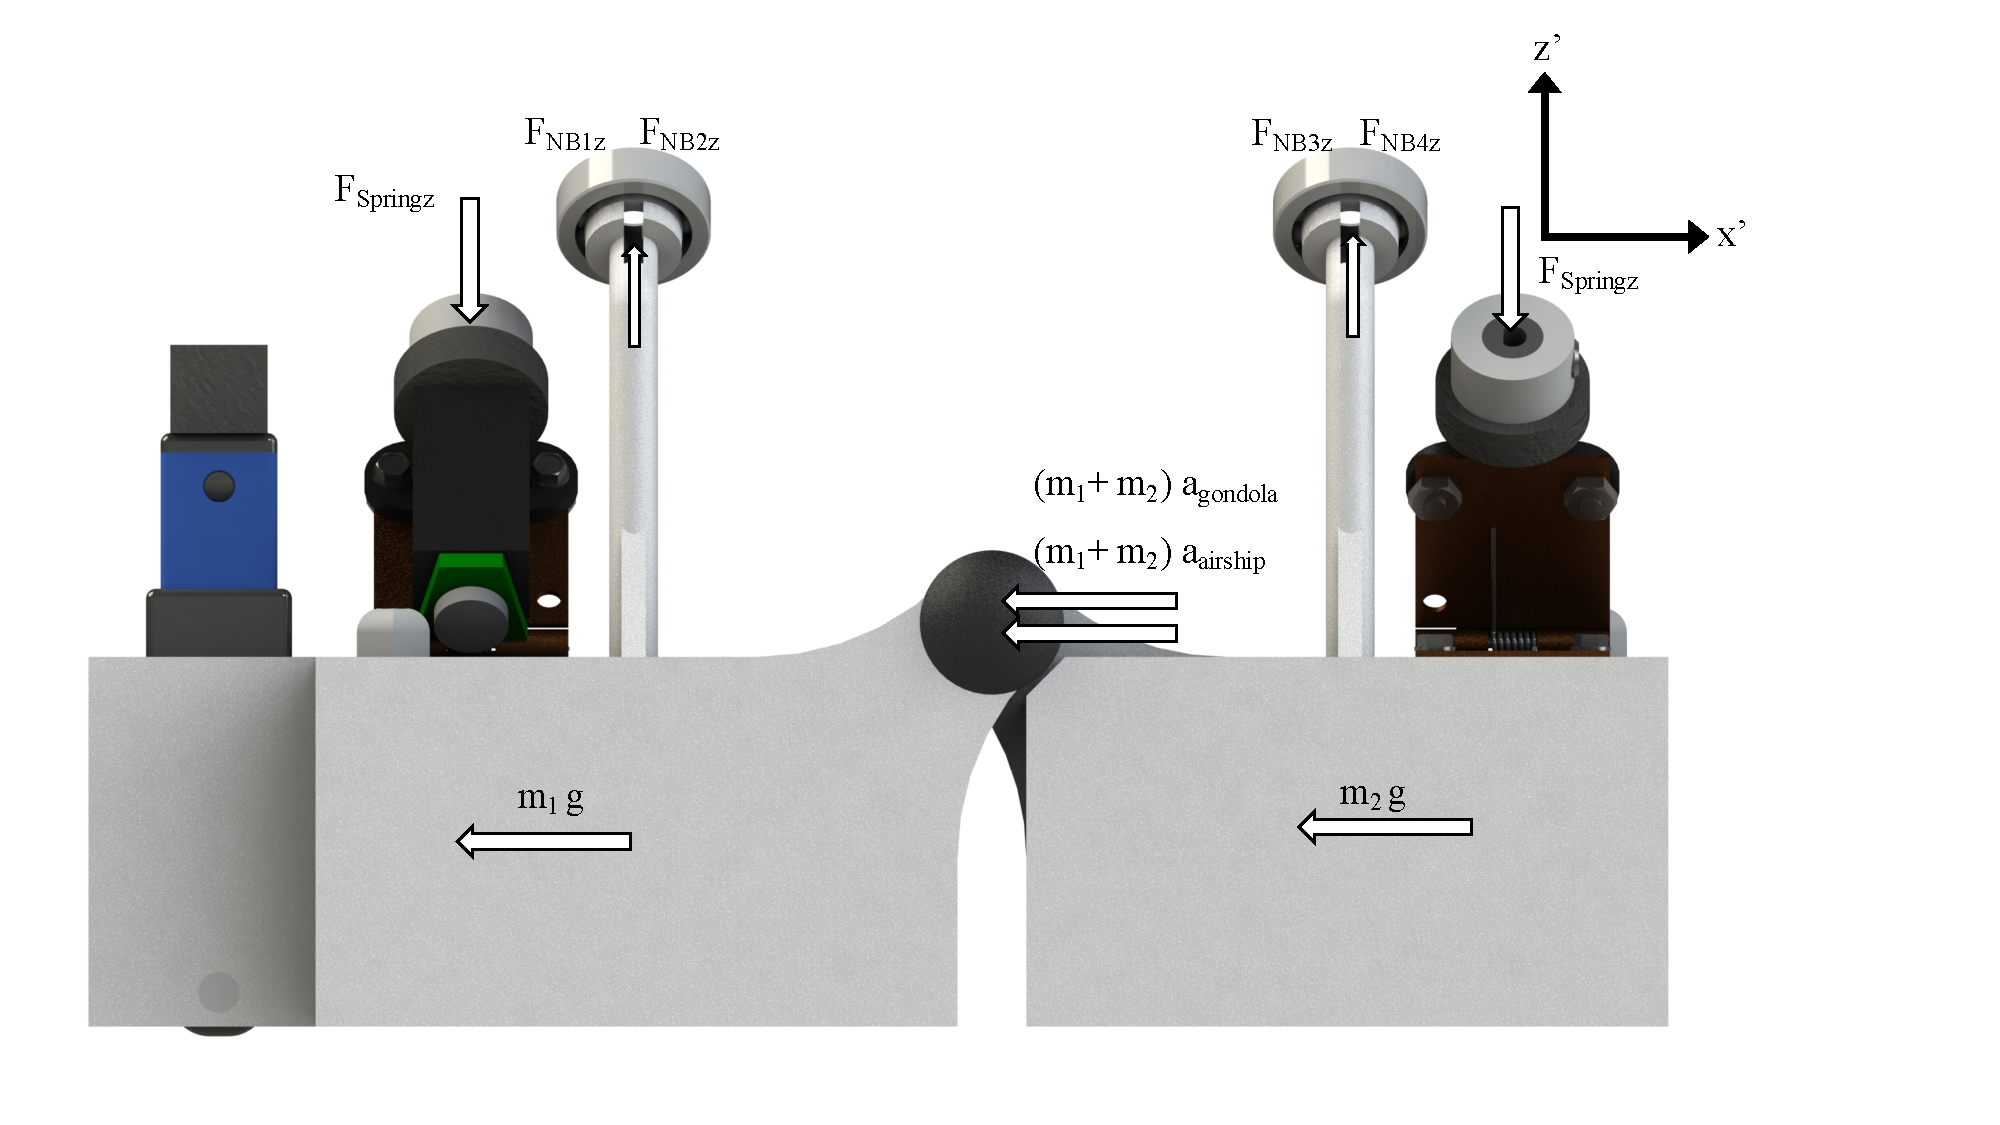
\includegraphics[width=1.1\textwidth]{img/gondola/sideGondolaNoDrive.pdf}
	\caption{Side View of Gondola With Linear Actuator Applied and No Drive Force}
	\label{fig:sideGondolaLA}
\end{figure}
 The sum of forces acting on the gondola are shown below in Equations \ref{eqn:FygondLA} and \ref{eqn:FzgondLA}. 
\begin{equation} \label{eqn:FygondLA}
\Sigma F_{y} : F_{NB1_{y}} - F_{NB2_{y}} - F_{NB3_{y}} + F_{NB4_{y}} = \frac{\sqrt{2}}{2} F_{Spring} -\frac{\sqrt{2}}{2} F_{Spring} 
\end{equation}
\begin{multline} \label{eqn:FzgondLA}
\Sigma F_{z} : F_{NB1_{z}} + F_{NB2_{z}} + F_{NB3_{z}} + F_{NB4_{z}} =\\ (m_{1} + m_2)g - \frac{\sqrt{2}}{2} F_{Spring} - \frac{\sqrt{2}}{2} F_{Spring} + \sin(\beta) (m_1+m_2) a_{Thrust}
\end{multline}
 
The sum of forces in the x direction are not shown because in this scenario, there are no forces acting in the x direction although the brake is applied. If there where any forces in the x direction since the brake is activated it would resisted by the braking force $F_{brake}$. The arm that is subjected to the highest force is usually located opposite to the friction wheel, but the code REF??? will check all the bearing forces, $F_{NB}$, and determine which is the largest. \\

The member is most likely fail at the inner interface with the gondola, marked as shown ing FIGURE ???. This is due to the fact that this corner will be in tension. Stress is only relevant acting upon the direction of anticipated rotation, in the x-direction. Stress at the inner corner of the arm is found as:

\begin{align}
	\sigma _{Gondola Arm} = \sigma _{axial} + \sigma _{bending force} + \sigma _{bending moment} \\ \label{armStress}
	\sigma _{Gondola Arm}  = \left(\dfrac{F_{NB_{z}}}{A}\right)\hat{k} + \left(\dfrac{F_{NB_{y}}l_{arm}c}{I}  + \dfrac{M_{NB}c}{I} \right) \hat{j}
\end{align}

These stresses are converted to principle stresses (as shown in Appendix \ref{appendix:cauchy}). These principle stresses are then used to determine the safety factor by Brittle Mohr-Coulomb Theory \cite[227]{shigley}.

Since $\sigma _a > \sigma _b > 0$,

\begin{equation}
	\eta = \dfrac{S_{ut}}{\sigma _a} \Rightarrow 1.5 \geq \dfrac{S_{ut}}{\sigma _a}
\end{equation}

\end{document}